\documentclass{article}
\usepackage[a4paper, margin=2.5cm, headheight=13pt]{geometry}
\usepackage[french]{babel}
\usepackage{fancyhdr}
\usepackage{tikz}
\usepackage{xcolor}
\usetikzlibrary{positioning, calc}
\usepackage{graphicx}

%define_color
\definecolor{bleu}{rgb}{0,0.52,1}
\definecolor{vert}{rgb}{0.45,0.82,0}

% Subfigures
\usepackage{caption}
\usepackage{subcaption}

% Définir la pagination etc.
\pagestyle{fancy}
\fancyhf{}
\lhead{MICRO-315 Miniprojet} 
\rhead{Les aventures de Jean-Bot}
\fancyfoot
{
    \begin{tikzpicture}[remember picture,overlay]
            \node[] (chat) at ($(current page.south)+(0,1.5)$) {
\includegraphics[width=1cm]{images/amour.pdf}};
            \node[] () at ($(chat)+(0,0.04)$) {\thepage};
            \node[] () at ($(chat)-(1,0)$) {
\includegraphics[width=1cm]{images/kawwai.pdf}};
            \node[] () at ($(chat)+(1,0)$) {\scalebox{-1}[1]{
\includegraphics[width=1cm]{images/kawwai.pdf}}};
    \end{tikzpicture}
}

\begin{document}
    \begin{titlepage}
        \vspace*{\fill}
        \begin{center}
            \begin{tikzpicture}[remember picture, overlay]
                \node[] at (current page.center) {\includegraphics[angle=90, width=\paperwidth]{images/background.jpg}};
                \fill[color = white, opacity = 0.9, rounded corners = 2ex] (-10,5) rectangle (10,-5);
                \node (titre) at (0,0)
                    {
                        \begin{tabular}{c}
                            \hline
                            \\
                            \huge\it Les aventures incroyables de \\
                            \\
                            \Huge\bf Jean-Bot Baptiste I\\
                            \\
                            \huge\it Le raccourceur des circuits\\
                            \\
                            \hline
                        \end{tabular}
                    };
                \node[left]  at (titre.west) {
\includegraphics[width=5cm]{images/kawwai.pdf}};
                \node[right] at (titre.east) {\scalebox{-1}[1]{
\includegraphics[width=5cm]{images/kawwai.pdf}}};
                \node[above] at (titre.north) {\textbf{\large MICRO-315 Miniprojet}};
                \node[below] at (titre.south) {\textit{\large Un projet de robotique de Julian Donevsky et Olof Lissmats}};
            \end{tikzpicture}
        \end{center}
        \vspace{5cm}
        \vspace*{\fill}
    \end{titlepage}

    \thispagestyle{empty}

    \tableofcontents

    \newpage

    \setcounter{page}{1}

    \section{Introduction}

    Dans le cadre de ce projet, nous avons créer un programme qui permet au robot de danser sur une musique en particulier en fonction d'un drapeau de pays que l'utilisateur lui présente. Le robot utilise ses capteurs de proximités infrarouges pour s'assurer qu'aucun obstacle ne bloque son chemin lorsqu'il danse. Si c'est le cas, il arrête temporairement sa danse jusqu'à ce que l'obstacle soit dégagé.

    \section{Métholodogie}
    
    \subsection{Schéma général du programme}
    \begin{figure}[!ht]
    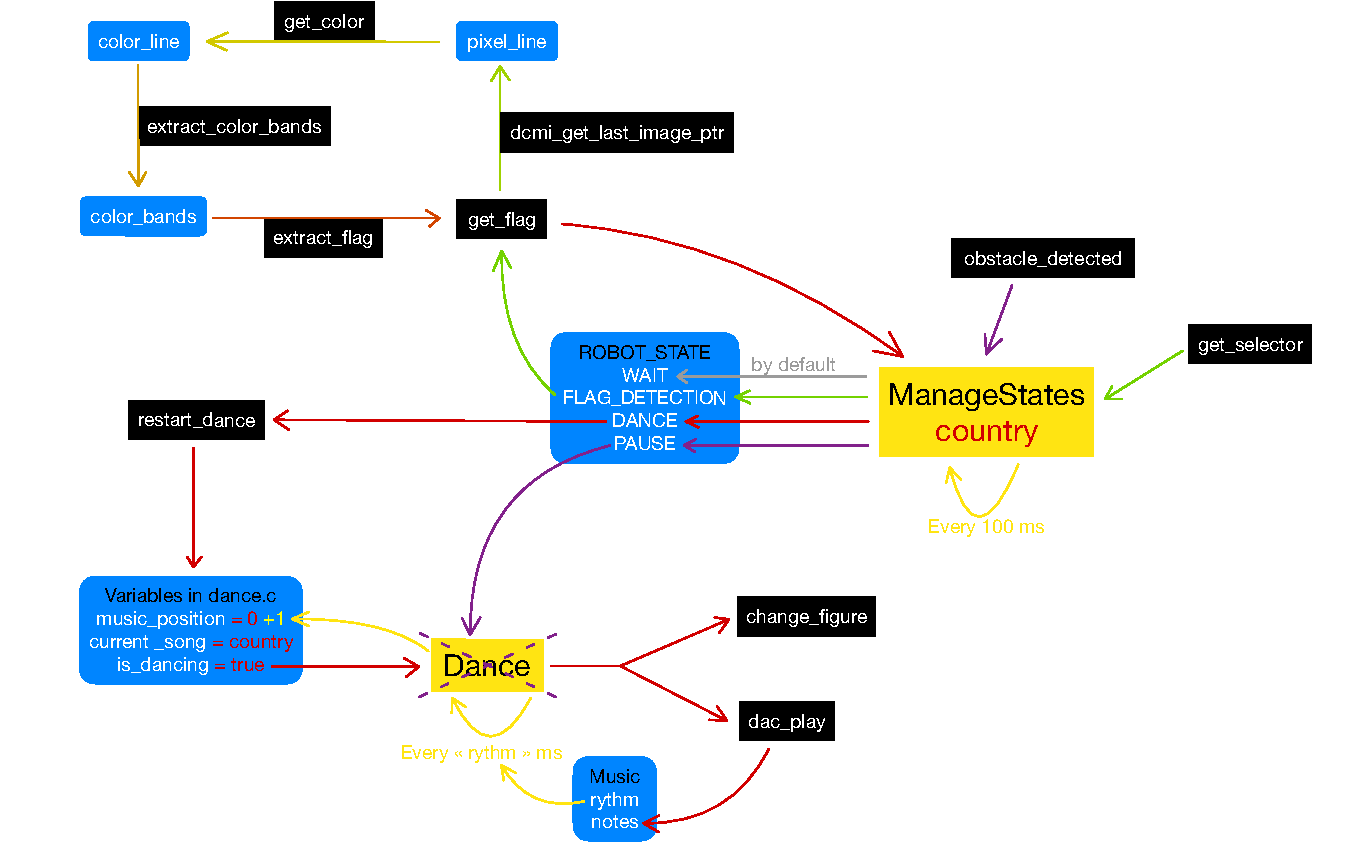
\includegraphics[scale=0.75]{docs/rapport/images/Structure_Code.pdf}
    \caption{Schéma général du programme. En jaune les threads, en noir les fonctions et en bleu (rouge dans le cas de country) les variables utiles au bon déroulement du programme.}
    \label{fig:structure} % Pour référer à cette figure dans le texte
\end{figure}

    L'utilisateur tourne le selecteur (peu importe de combien de cran). En appellant la fonction \textbf{get$\_$selector}, le thread \colorbox{yellow}{\textbf{ManagesStates}} met l'état du robot à \textcolor{bleu}{FLAG$\_$DETECTION} ce qui a pour conséquence d'appeler la fonction \textbf{get$\_$flag} (\textcolor{vert}{flèche en vert}). \par
    
    A chaque appel de \textbf{get$\_$flag}, une image sur la caméra est capturée et on stocke une ligne de pixel dans la variable \textcolor{bleu}{pixel$\_$line}. On convertit chaque pixel de \textcolor{bleu}{pixel$\_$line} en un pixel de couleur (blanc, rouge, vert, bleu, indéfini) grâce à la fonction \textbf{get$\_$color} qu'on stocke ensuite dans \textcolor{bleu}{color$\_$line}. La fonction \textbf{extract$\_$color$\_$bands} s'occupe d'analyser \textcolor{bleu}{color$\_$line} (voir section \ref{extract_color_bands}) pour 

    \subsection{La fonction extract$\_$color$\_$bands}
    \label{extract_color_bands}
    \begin{figure}[!ht]
        \centering
        \begin{subfigure}{\textwidth}
            \begin{center}
                \begin{tikzpicture}[scale=0.3]
                    \foreach \i in {1,...,4}
                    {
                        \draw[fill=gray] (\i,0) rectangle (\i+1,2);
                    }
                    \foreach \i in {5,...,8}
                    {
                        \draw[fill=red] (\i,0) rectangle (\i+1,2);
                    }
                    \foreach \i in {9,...,11}
                    {
                        \draw[fill=green] (\i,0) rectangle (\i+1,2);
                    }
                    \foreach \i in {12,...,13}
                    {
                        \draw (\i,0) rectangle (\i+1,2);
                    }
                    \foreach \i in {14,...,23}
                    {
                        \draw[fill=blue] (\i,0) rectangle (\i+1,2);
                    }
                    \foreach \i in {24,...,27}
                    {
                        \draw (\i,0) rectangle (\i+1,2);
                    }
                    \draw[fill=green] (28,0) rectangle (29,2);
                    \foreach \i in {29,...,34}
                    {
                        \draw (\i,0) rectangle (\i+1,2);
                    }
                    \foreach \i in {35,...,44}
                    {
                        \draw[fill=red] (\i,0) rectangle (\i+1,2);
                    }
                \end{tikzpicture}
            \end{center}
            \caption{Une fois les valeurs RGB de chaque pixel sont convertits à des couleurs, elles sont stockées de cette manière. La couleur grise représente une couleur non définie. La caméra fournit en fait une ligne de 640 pixels, mais dans cet exemple seulement 40 sont représentés.}
        \end{subfigure}

        \vspace{5mm}

        \begin{subfigure}{\textwidth}
            \begin{center}
                \begin{tikzpicture}[scale=0.4]
                    \draw[fill=gray]  (0,3) rectangle (1,5) node[midway] (A) {};
                    \draw[fill=red]   (1,3) rectangle (2,5);
                    \draw[fill=green] (2,3) rectangle (3,5);
                    \draw[fill=white] (3,3) rectangle (4,5);
                    \draw[fill=blue]  (4,3) rectangle (5,5);
                    \draw[fill=white] (5,3) rectangle (6,5);
                    \draw[fill=green] (6,3) rectangle (7,5);
                    \draw[fill=white] (7,3) rectangle (8,5);
                    \draw[fill=red]   (8,3) rectangle (9,5);
                    \node[anchor=east] () at ($(A)-(1,0)$) {\texttt{color\_groups:}};

                    \draw (0,0) rectangle (1,2) node[midway] (B) {\texttt{4}};
                    \draw (1,0) rectangle (2,2) node[midway] {\texttt{4}};
                    \draw (2,0) rectangle (3,2) node[midway] {\texttt{3}};
                    \draw (3,0) rectangle (4,2) node[midway] {\texttt{2}};
                    \draw (4,0) rectangle (5,2) node[midway] {\texttt{10}};
                    \draw (5,0) rectangle (6,2) node[midway] {\texttt{4}};
                    \draw (6,0) rectangle (7,2) node[midway] {\texttt{1}};
                    \draw (7,0) rectangle (8,2) node[midway] {\texttt{6}};
                    \draw (8,0) rectangle (9,2) node[midway] {\texttt{10}};
                    \node[anchor=east] () at ($(B)-(1,0)$) {\texttt{size\_of\_groups:}};
                \end{tikzpicture}
            \end{center}
            \caption{Les pixels sont groupés en fonction de leurs couleurs dans les deux arrays \texttt{color\_groups} et \texttt{size\_of\_groups} qui contiennent la couleur et la taille des groupes respectivement.}
        \end{subfigure}

        \vspace{5mm}

        \begin{subfigure}{\textwidth}
            \begin{center}
                \begin{tikzpicture}[scale=0.4]
                    \draw[fill=gray]  (0,3) rectangle (1,5) node[midway] (A) {};
                    \draw[fill=red]   (1,3) rectangle (2,5);
                    \draw[fill=blue]  (2,3) rectangle (3,5);
                    \draw[fill=white] (3,3) rectangle (4,5);
                    \draw[fill=white] (4,3) rectangle (5,5);
                    \draw[fill=red]   (5,3) rectangle (6,5);
                    \draw[fill=gray]  (6,3) rectangle (7,5);
                    \node[anchor=east] () at ($(A)-(1,0)$) {\texttt{color\_groups:}};

                    \draw (0,0) rectangle (1,2) node[midway] (B) {\texttt{4}};
                    \draw (1,0) rectangle (2,2) node[midway] {\texttt{4}};
                    \draw (2,0) rectangle (3,2) node[midway] {\texttt{10}};
                    \draw (3,0) rectangle (4,2) node[midway] {\texttt{4}};
                    \draw (4,0) rectangle (5,2) node[midway] {\texttt{6}};
                    \draw (5,0) rectangle (6,2) node[midway] {\texttt{10}};
                    \draw (6,0) rectangle (7,2) node[midway] {\texttt{?}};
                    \node[anchor=east] () at ($(B)-(1,0)$) {\texttt{size\_of\_groups:}};
                \end{tikzpicture}
            \end{center}

            \caption{Les groupes avec une taille supérieur à une seuile spécifique, ici 3, sont placés au début des arrays, c'est à dire que les groupes trop petits sont supprimés. Cela se fait pour ammortir l'effet de bruit.}
        \end{subfigure}

        \vspace{5mm}

        \begin{subfigure}{\textwidth}
            \begin{center}
                \begin{tikzpicture}[scale=0.4]
                    \draw[fill=gray]  (0,3) rectangle (1,5) node[midway] (A) {};
                    \draw[fill=red]   (1,3) rectangle (2,5);
                    \draw[fill=blue]  (2,3) rectangle (3,5);
                    \draw[fill=white] (3,3) rectangle (4,5);
                    \draw[fill=red]   (4,3) rectangle (5,5);
                    \draw[fill=gray]  (5,3) rectangle (6,5);
                    \node[anchor=east] () at ($(A)-(1,0)$) {\texttt{color\_groups:}};

                    \draw (0,0) rectangle (1,2) node[midway] (B) {\texttt{4}};
                    \draw (1,0) rectangle (2,2) node[midway] {\texttt{4}};
                    \draw (2,0) rectangle (3,2) node[midway] {\texttt{10}};
                    \draw (3,0) rectangle (4,2) node[midway] {\texttt{10}};
                    \draw (4,0) rectangle (5,2) node[midway] {\texttt{10}};
                    \draw (5,0) rectangle (6,2) node[midway] {\texttt{?}};
                    \node[anchor=east] () at ($(B)-(1,0)$) {\texttt{size\_of\_groups:}};
                \end{tikzpicture}
            \end{center}

            \caption{Les groupes consécutives ayant la même couleur sont fusionnés, et les groupes suivants sont décalés d'un placement.}
        \end{subfigure}

        \vspace{5mm}

        \begin{subfigure}{\textwidth}
            \begin{center}
                \begin{tikzpicture}[scale=0.4]
                    \draw[fill=gray]  (0,3) rectangle (1,5) node[midway] (A) {};
                    \draw[fill=blue]  (1,3) rectangle (2,5);
                    \draw[fill=white] (2,3) rectangle (3,5);
                    \draw[fill=red]   (3,3) rectangle (4,5);
                    \draw[fill=gray]  (4,3) rectangle (5,5);
                    \node[anchor=east] () at ($(A)-(1,0)$) {\texttt{color\_groups:}};
                \end{tikzpicture}
            \end{center}

            \caption{Les groupes d'une taille inférieure d'une seuile spécifique, ici 8, sont fusionnés avec les groupes non-définis entourants.}
        \end{subfigure}
        \caption{Un schéma qui explique comment fonctionne la détection des drapeaux.}
    \end{figure}

\end{document}
